\documentclass[]{article}
\usepackage{lmodern}
\usepackage{amssymb,amsmath}
\usepackage{ifxetex,ifluatex}
\usepackage{fixltx2e} % provides \textsubscript
\ifnum 0\ifxetex 1\fi\ifluatex 1\fi=0 % if pdftex
  \usepackage[T1]{fontenc}
  \usepackage[utf8]{inputenc}
\else % if luatex or xelatex
  \ifxetex
    \usepackage{mathspec}
  \else
    \usepackage{fontspec}
  \fi
  \defaultfontfeatures{Ligatures=TeX,Scale=MatchLowercase}
\fi
% use upquote if available, for straight quotes in verbatim environments
\IfFileExists{upquote.sty}{\usepackage{upquote}}{}
% use microtype if available
\IfFileExists{microtype.sty}{%
\usepackage{microtype}
\UseMicrotypeSet[protrusion]{basicmath} % disable protrusion for tt fonts
}{}
\usepackage[margin=1in]{geometry}
\usepackage{hyperref}
\hypersetup{unicode=true,
            pdftitle={Models 1 - Herbivore biomass gradients},
            pdfborder={0 0 0},
            breaklinks=true}
\urlstyle{same}  % don't use monospace font for urls
\usepackage{graphicx,grffile}
\makeatletter
\def\maxwidth{\ifdim\Gin@nat@width>\linewidth\linewidth\else\Gin@nat@width\fi}
\def\maxheight{\ifdim\Gin@nat@height>\textheight\textheight\else\Gin@nat@height\fi}
\makeatother
% Scale images if necessary, so that they will not overflow the page
% margins by default, and it is still possible to overwrite the defaults
% using explicit options in \includegraphics[width, height, ...]{}
\setkeys{Gin}{width=\maxwidth,height=\maxheight,keepaspectratio}
\IfFileExists{parskip.sty}{%
\usepackage{parskip}
}{% else
\setlength{\parindent}{0pt}
\setlength{\parskip}{6pt plus 2pt minus 1pt}
}
\setlength{\emergencystretch}{3em}  % prevent overfull lines
\providecommand{\tightlist}{%
  \setlength{\itemsep}{0pt}\setlength{\parskip}{0pt}}
\setcounter{secnumdepth}{0}
% Redefines (sub)paragraphs to behave more like sections
\ifx\paragraph\undefined\else
\let\oldparagraph\paragraph
\renewcommand{\paragraph}[1]{\oldparagraph{#1}\mbox{}}
\fi
\ifx\subparagraph\undefined\else
\let\oldsubparagraph\subparagraph
\renewcommand{\subparagraph}[1]{\oldsubparagraph{#1}\mbox{}}
\fi

%%% Use protect on footnotes to avoid problems with footnotes in titles
\let\rmarkdownfootnote\footnote%
\def\footnote{\protect\rmarkdownfootnote}

%%% Change title format to be more compact
\usepackage{titling}

% Create subtitle command for use in maketitle
\newcommand{\subtitle}[1]{
  \posttitle{
    \begin{center}\large#1\end{center}
    }
}

\setlength{\droptitle}{-2em}

  \title{Models 1 - Herbivore biomass gradients}
    \pretitle{\vspace{\droptitle}\centering\huge}
  \posttitle{\par}
    \author{}
    \preauthor{}\postauthor{}
    \date{}
    \predate{}\postdate{}
  

\begin{document}
\maketitle

\paragraph{Report contains model outputs and diagnostics for grazing
biomass
models.}\label{report-contains-model-outputs-and-diagnostics-for-grazing-biomass-models.}

\paragraph{Predictor dataframe}\label{predictor-dataframe}

We expect herbivore biomass to be predicted by hard coral cover,
macroalgal cover, complexity, and fishing pressure. These 4 covariates
are not correlated (Figure 1), so models will not be biased by
collinearity issues. We are scaling covariates to a mean of 0 and
standard deviation of 1, which is recommended for multimodel selection
approaches, and allows for meaningful comparisons of effect sizes when
covariates are on different scales (e.g.~benthic cover \% vs.~habitat
complexity).

Additional covariates to consider may be disturbance history, oceanic
productivity, and wave energy (Heenan et al. 2016, Proceedings), but
these are probably not available for all UVC sites.

\begin{figure}
\centering
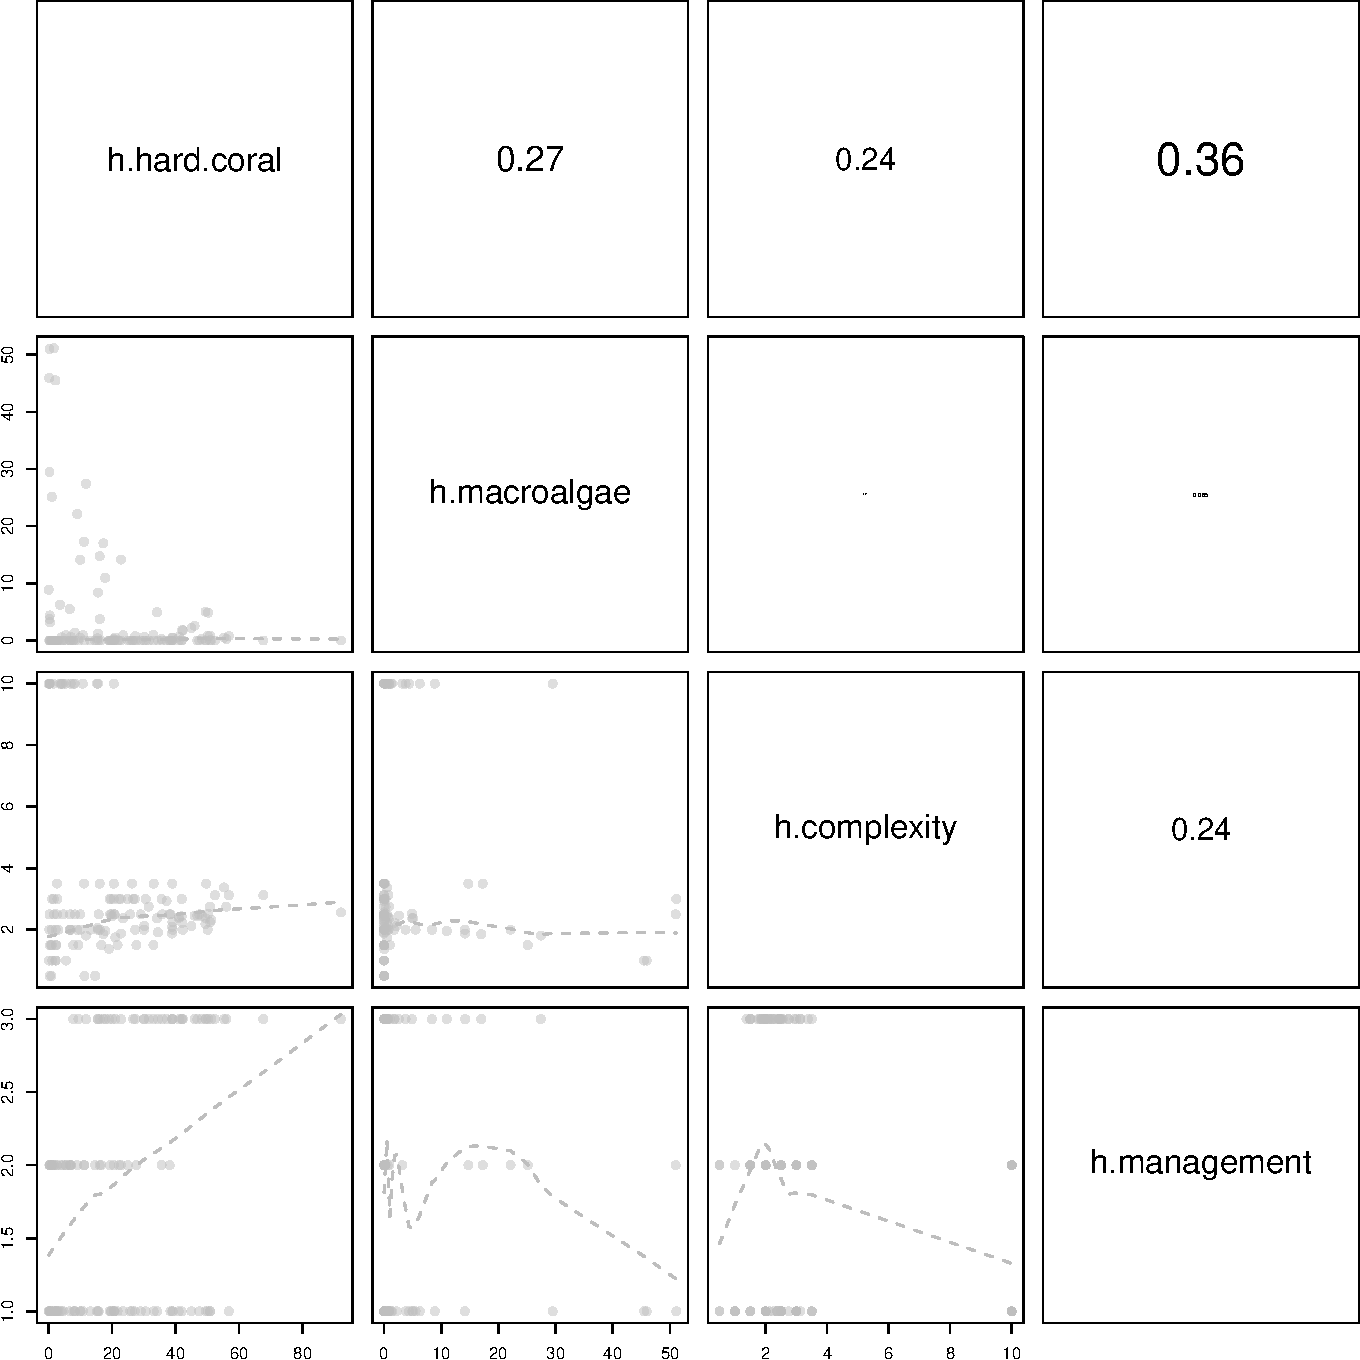
\includegraphics{01_biomass_models_files/figure-latex/unnamed-chunk-2-1.pdf}
\caption{Correlation between unscaled explanatory covariates}
\end{figure}

\newpage

\subsection{Grazer models}\label{grazer-models}

~

Now fitting models to grazers, with scaled continuous covariates and
dummy categorical covariates. We will account for non-independence of
islands and sites (i.e.~correlated biomass estimates within a region)
with random effect structures.

Fitted model is:

grazerlog10 \textasciitilde{} fixed(hard.coral + macroalgae * complexity
+ fished + pristine) + random(dataset/reef)

where grazerlog10 is grazer biomass (log10 scale), fished indicates if a
site is protected or fished, and pristine indicates if a site is
pristine (i.e.~remote Chagos reefs). Random effect is varying intercepts
for each reef, nested in each dataset.

\begin{figure}
\centering
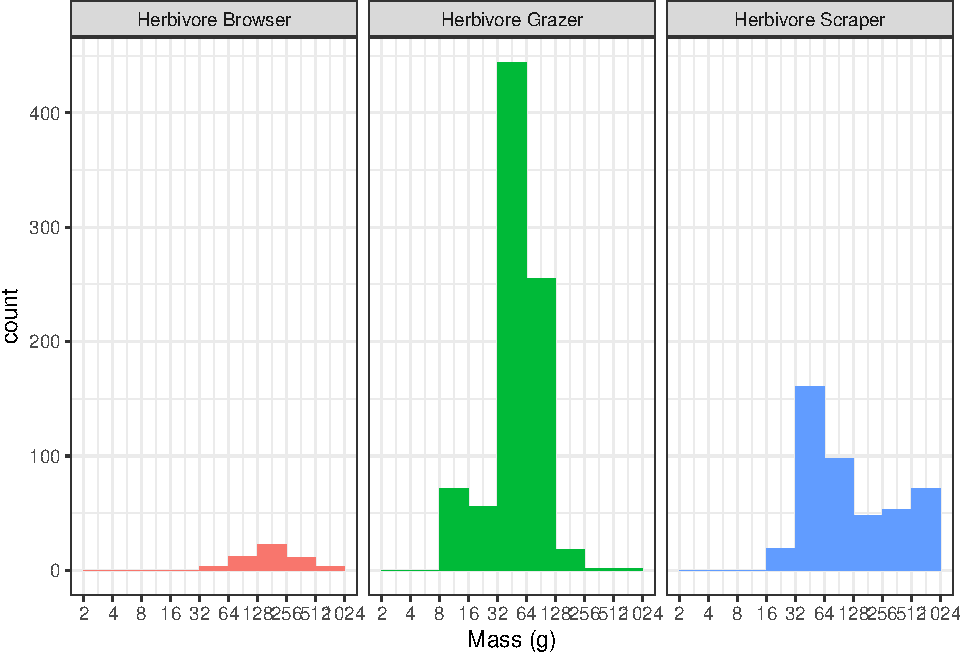
\includegraphics{01_biomass_models_files/figure-latex/unnamed-chunk-6-1.pdf}
\caption{Grazer model diagnostics - residuals and fitted values}
\end{figure}

Model residuals are approx. normal (though fail a shapiro test), while
model predictions are reasonable. Note clustering of predictions around
1-2 observed biomass. Suggests that commonly-observed biomass values are
not well predicted by habitat or fishing. Also note positive residual
relationship, indicating that small biomass values are underpredicted
and large biomass are overpredicted.

Next step, examing model estimated effects by visualizing change in
biomass across observed gradients in explanatory covariates.

\newpage

\paragraph{Benthic effects}\label{benthic-effects}

\begin{figure}
\centering
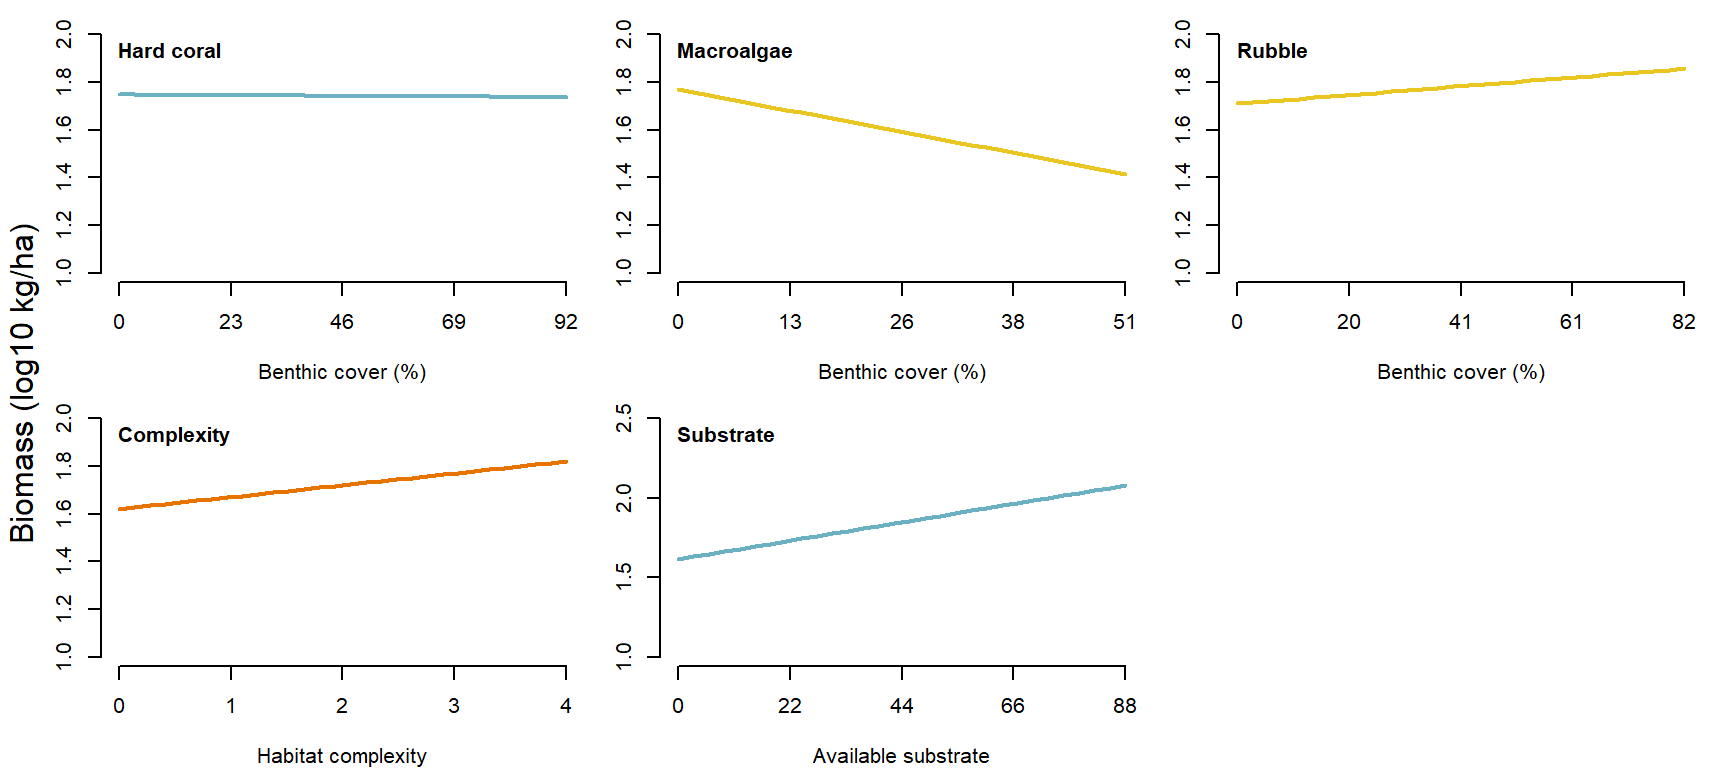
\includegraphics{01_biomass_models_files/figure-latex/unnamed-chunk-8-1.pdf}
\caption{Grazer model effects}
\end{figure}

\begin{itemize}
\item
  Macroalgae has the strongest effect on grazer biomass, which declined
  from \texttt{50} kg/ha at 0\% cover to \texttt{19} kg/ha at
  \texttt{51} \% cover.
\item
  Complexity has a moderate effect on grazer biomass, which increased
  from \texttt{45} kg/ha at 0\% cover to \texttt{50} kg/ha at
  \texttt{10} complexity.
\item
  Hard coral has the weakest effect on grazer biomass, which increased
  from \texttt{45} kg/ha at 0\% cover to \texttt{51} kg/ha at
  \texttt{92} \% cover.
\end{itemize}

\newpage

\paragraph{Fishing effects}\label{fishing-effects}

\begin{figure}
\centering
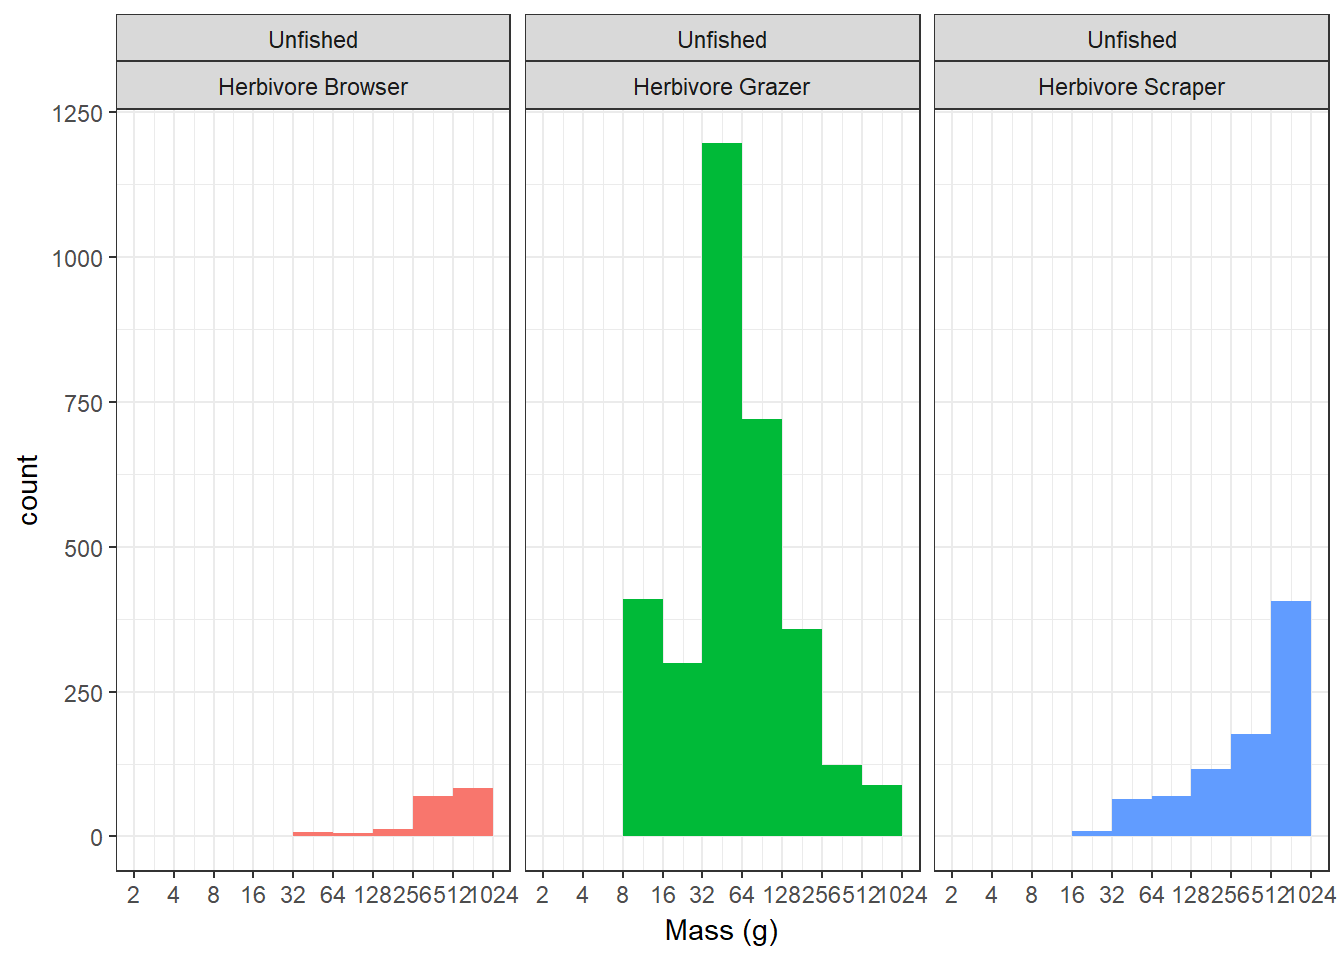
\includegraphics{01_biomass_models_files/figure-latex/unnamed-chunk-10-1.pdf}
\caption{Predicted grazer biomass across fishing gradient}
\end{figure}

\begin{itemize}
\item
  Pristine reefs have the highest grazer biomass, at \texttt{213} kg/ha.
\item
  Protected and fished reefs have similar biomass levels, at \texttt{47}
  kg/ha on protected reefs and \texttt{43} kg/ha on fished reefs.
\end{itemize}

\newpage

\subsubsection{Browsers}\label{browsers}

~

Y'all ready for this?


\end{document}
